\documentclass[conference]{IEEEtran}
\usepackage{cite}
\usepackage{amsmath,amssymb,amsfonts}
\usepackage{algorithmic}
\usepackage{booktabs}
\usepackage{caption}
\usepackage{graphicx}
\usepackage{listings}
\usepackage{textcomp}
\usepackage{xcolor}
\def\BibTeX{{\rm B\kern-.05em{\sc i\kern-.025em b}\kern-.08em
    T\kern-.1667em\lower.7ex\hbox{E}\kern-.125emX}}
\begin{document}


\title{CENG435 Term Project, Part 1\\
}

\author{\IEEEauthorblockN{Doruk Coskun}
\IEEEauthorblockA{
}
\and
\IEEEauthorblockN{Yagmur Oymak}
\IEEEauthorblockA{
}
}

\maketitle

\section{Introduction}

In our CENG435 Term Project Part 1 we have designed a network topology according to the information provided to us in the homework description. We have formed a TCP connection between Source and Broker. We implemented UDP connection between Broker, Router 1, Router 2 and Destination. We tested packet loss and packet delays in our network.

\section{Setting Up the Environment}
To set network emulation delays, \textbf{tc} command is used. \textbf{tc} manipulates
traffic control parameters in a Linux system. Running verbose \textbf{tc} commands
in multiple machines becomes tedious very quickly.
In order to quickly and conveniently set delays in multiple nodes and multiple links,
we've used the shell scripts mentioned in the README file.

Likewise, short shell scripts were used for placing the code files in relevant
nodes.

\section{Network Topology Design Decisions}

In our design, packet sent from Source passes through Broker, Router 1 and reaches Destination. All scripts except Broker is written in Python3. Before the packet is sent a TCP connection formed between Source and Broker. Our sensor readings are 8 bytes long and consists of the index of the packet. We have chosen this packet size so that we can can minimize the transmission delay and observe the netem/tc delays better. When the byte stream reaches Broker, they are sent to Router 1 through UDP connection. Router 1 listens to a predefined port number and directs the packet to Destination. Destination prints out the content of the received packet and sends feedback back to the source through Router 2. Router 2 directs the packet received from Destination to Broker. Finally broker uses the already open TCP connection to send the feedback message to Source. Source calculates the time difference between the sent packet and the received feedback message. By this method we have calculated the round-trip time. We have also implemented a method where we have synchronized the nodes and calculated the one way delay using time stamps that are sent with the packets. But we believe we have gathered more accurate results using round-trip time. You can find detailed synchronization implementation in the following parts of this documentation.

\subsection{Packet Loss Test}\label{AA}

Apart from delay tests we have also implemented packet loss test. In this test we have sent 1000 consecutive packets from Source and observed how many of them reached to Broker and then to Destination. Its important to keep in mind that our packet size is 8 bytes. 
\begin{itemize}
\item 1000/1000: All of the packets sent by Source were received by Broker. Since the connection between Source and Destination is TCP, packet loss is not expected.
\item 67/1000: Only 67 of the packets were received by the destination. There is a significant packet loss. We exceed the capacity of the links between the other nodes. That's why while transferring the packets through UDP nodes, most of them were lost. While we were sending packets of size 128 bytes, the packet loss rate was even higher, with only 17 packets reaching Destination. We also observed that when we increased the size of the packets to 4 times, the amount of the packets delivered to Destination reduced to 1 over 4.
\end{itemize}

\subsection{Detailed Explanation of Synchronized Nodes}
As previously mentioned, we approximate the end-to-end delay using the round trip time, i.e.\
end-to-end delay is round trip time divided by two. Since our network delays will
most likely be symmetric, this approach deemed to be accurate enough. Still,
we implemented an alternative method of calculating the end-to-end delay using
timestamps in packets. For this approach to produce reliable results, the clocks
of the source and the destination must be synchronized.

In order to synchronize the nodes, \textbf{NTP} is used. NTP sets the clock of the
node using information from a time server. The following command is used to set the
clock of the node:
\begin{lstlisting}
sudo ntpdate -s time.nist.gov
\end{lstlisting}
Then, the \textbf{clockdiff} program can be used to calculate the clock difference
of two nodes. \textbf{clockdiff} uses ICMP TIMESTAMP packets (RFC0792, page 16)
to measure the clock difference of two hosts with a 1ms resolution. An example run:
\begin{lstlisting}
yagmuroy@d:~\$ clockdiff 172.17.1.7.
host=172.17.1.7 rtt=750(187)ms/0ms
delta=-277ms/-277ms Wed Nov 28 11:55:06 2018
\end{lstlisting}
When the clock difference (delta) became small (around 5ms), we ran our experiments.
Not to our surprise, the measured delay value was very close to our other approximation
(round trip time divided by two). For practical purposes\footnote{Even though the nodes had been
synchronised, their clocks started to drift and introduced noise in our measurements
before any meaningful data was collected.}, we deemed it appropriate
to use the round trip time approximation instead of the timestamp method.

\subsection{Detailed Explanation of Broker Implementation}
The broker is implemented as a multi-process server in C. This section describes
the implementation of the broker from a high level viewpoint.

The broker, when started, creates a TCP socket, binds it to a local port, and listens
it. It also creates two UDP sockets, one to send datagrams to Router 1, and one to receive
datagrams from Router 2. Since the first UDP socket will always send datagrams to a
fixed address and port (identifying the receiving socket at Router 1), we also
call connect on the socket to save us from specifying the address and port at every send call.
The second will receive datagrams from Router 2, therefore it must wait for packets
on a fixed port (the port that Router 2 will send to). So it also binds the socket
to a local address and port.

After the sockets are created, connected, bound and listened, the broker starts
its main loop in which it accepts TCP connections with the accept system call.
When the Source connects to the broker, a new worker process is spawned. This worker
process will handle the TCP connection socket. It receives byte streams from the Source,
packetizes the bytes and sends them to Router 1 using the previously
created UDP sockets. It also spawns another worker process (which shares the connection
socket) that receives datagrams (containing feedback messages) from Router 2 and
sends them over the TCP connection socket to the Source.

When the TCP connection from the source is terminated, the recv call will return 0
to the broker indicating connection termination. Knowing the connection is closed,
the worker process kills its child (the other worker process that it spawned),
checks if there is any leftover data coming from Router 2, clears it if there is
and exits. The main process still waits to accept new TCP connections, so the broker
is a server that always keeps running.

\section{Experiments}

In our experiments we have plotted the 3 scenarios given in the homework text:

\begin{itemize}
    \item \textbf{Experiment 1:} 1ms $\pm$ 5ms
    \item \textbf{Experiment 2:} 20ms $\pm$ 5ms
    \item \textbf{Experiment 3:} 60ms $\pm$ 5ms
\end{itemize}
You can find end-to-end delay results of these experiments in Figure~\ref{fig:graph}.

Apart from these experiments we have also observed the end-to-end delay without any network delay emulations. In the first glance we could not make much sense of the results. That's why we have concluded to  make even more test with different emulated network delays and compare those results. Remaining experiments, their mean delays, jitter delays and the estimated end-to-end delay can be seen below:

\begin{itemize}
    \item \textbf{Experiment 0:} 0 emulated delay, end-to-end delay: 20ms
    \item \textbf{Experiment 4:} 1ms $\pm$ 1 ms, end-to-end delay: 20ms
    \item \textbf{Experiment 5:} 5ms $\pm$ 1ms, end-to-end delay: 20ms
    \item \textbf{Experiment 6:} 7.5ms $\pm$ 1ms, end-to-end delay: 20ms
    \item \textbf{Experiment 7:} 10ms $\pm$ 1ms, end-to-end delay: 20ms
    \item \textbf{Experiment 8:} 12.5ms $\pm$ 1ms, end-to-end delay: 25ms
    \item \textbf{Experiment 9:} 15ms $\pm$ 1ms, end-to-end delay: 30ms
    \item \textbf{Experiment 10:} 20ms $\pm$ 1ms, end-to-end delay: 40ms
    \item \textbf{Experiment 11:} 50ms $\pm$ 1ms, end-to-end delay: 100ms
    \item \textbf{Experiment 12:} 100ms $\pm$ 1ms, end-to-end delay: 200ms
\end{itemize}

For our experiments we have first set the network emulation delays. We have collected the end-to-end delay data of 1100 packets for each experiment. Using these data we have found the mean delays and 95\% confidence interval.

Figure~\ref{fig:graph} illustrates our experimental results.
We calculated the 95\% confidence intervals as 19.2 to 19.6 for Experiment 0,
19.1 to 19.7 for Experiment 1, 40.6 to 41.2 for Experiment 2 and 120.9 to 121.1
for Experiment 3.

In the light of all the experiments, we have concluded that when the netem/tc delay is set lower than the actual end-to-end delay, it does not effect the end-to-end delay of the packets. We observed looking at the Experiments 1, 4, 5, 6, and 7 that end-to-end delay remains the same even though netem/tc delay was increased gradually but did not exceed the actual end-to-end delay. When, the netem/tc delay is bigger than the actual end-to-end delay, netem/tc delay is not added on the top of the actual delay but it extends the delay at the each node to the set amount as it can be seen in the Experiments 8, 9, 10, 11 and 12. Since the delay between Source and Broker is negligible (Link capacity is 100 times of the other links in the network) netem/tc delay set on the UDP nodes, determine the total end-to-end delay.

\begin{figure}
    \centering
    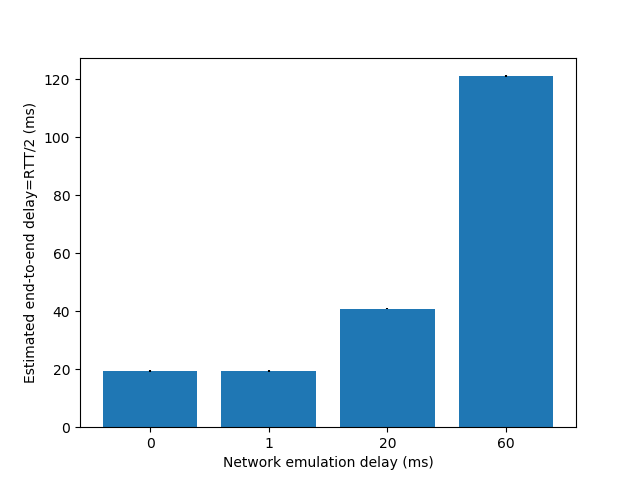
\includegraphics[scale=0.6]{graphics/plt}
    \caption{Network emulation delay vs.\ end-to-end delay}\label{fig:graph}
\end{figure}

Having read the manual of netem/tc we had hard time making sense about the results we got from the experiments. We were expecting to see our end-to-end delay to increase by network emulation delay for each network delay emulated node. Namely for each pass through broker and router. As an example when we set netem/tc delay to 20ms with 5ms jitter we expected to see the delay: $20ms$ (actual delay) $+$ $20ms$ (delay from broker) $+$ $20ms$ (delay from router 1) $=$ $60ms$.

Moreover, with or without emulated delays, the first few packets sent would return
very quickly (in the order of a few milliseconds) but as the source sent more packets,
the delay would quickly increase to a higher value (around 39 milliseconds with no
emulated delay). To make sense of this, we ran some experiments using \textbf{ping}
with different packet sizes and time intervals. Curiously, a similar pattern was observed
with certain configurations; first few packets would arrive in a few milliseconds, then
after a point, packets would be delayed and started to drop. This may be interpreted
as the link capacity being exceeded; however this should not have happened in our test programs
because the source does not send any new packets until the feedback of the last packet it had sent
returned. The source should not be able to congest the link, yet it does
(or an implementation error we could not detect causes this strange pattern).

Figure~\ref{fig:graph} illustrates our experimental results.
We calculated the 95\% confidence intervals as 19.2 to 19.6 for experiment 0,
19.1 to 19.7 for experiment 1, 40.6 to 41.2 for experiment 2 and 120.9 to 121.1
for experiment 3. Table~\ref{table:data} shows the summary of the results.\\

\begin{table}
    \centering
    \begin{tabular}{c c c c}
        \toprule
        NetEm delay & $\mu$ & $\sigma$ & Error \\
        $0ms$   &    $19.4ms$   &   $3.43ms$    &   $0.203ms$ \\
        $1ms$   &    $19.4ms$   &   $4.47ms$    &   $0.264ms$ \\
        $20ms$   &    $40.9ms$   &   $4.92ms$    &   $0.291ms$ \\
        $60ms$   &    $121ms$   &   $4.99ms$    &   $0.295ms$ \\
        \bottomrule
    \end{tabular}\label{table:data} \\
    \caption{Summary of experimental data}\label{table:data}
\end{table}

\end{document}
